\documentclass[oneside,14pt]{extarticle}
\usepackage{cmap}
\usepackage[utf8]{inputenc}
\usepackage[english,ukrainian]{babel}
\usepackage{graphicx}
\usepackage{geometry}
\usepackage{listings}
\usepackage{float}
\usepackage{amsmath}
\usepackage{subfig}
\geometry{
	a4paper,
	left=20mm,
	right=20mm,
	top=15mm,
	bottom=15mm,
}
\lstset{
	language=c,
	tabsize=4,
	keepspaces,
	showstringspaces=false,
	frame=single,
	breaklines,
	language=C,
}
\graphicspath{ {./pictures} }
\setlength{\parindent}{4em}

\newcommand\subject{Основи програмування вбудованих систем}
\newcommand\lecturer{доцентка кафедри ПЗ\\Марусенкова Т.А.}
\newcommand\teacher{доцент кафедри ПЗ\\Крук О.Г.}
\newcommand\mygroup{ПЗ-32}
\newcommand\lab{7}
\newcommand\theme{Мапування пам'яті та робота зі scatter-файлом}
\newcommand\purpose{Навчитися використовувати можливості лінкувальника та розташовувати дані за потрібними адресами}

\begin{document}
\begin{normalsize}
	\begin{titlepage}
		\thispagestyle{empty}
		\begin{center}
			\textbf{МІНІСТЕРСТВО ОСВІТИ І НАУКИ УКРАЇНИ\\
				НАЦІОНАЛЬНИЙ УНІВЕРСИТЕТ "ЛЬВІВСЬКА ПОЛІТЕХНІКА"}
		\end{center}
		\begin{flushright}
			\textbf{ІКНІ}\\
			Кафедра \textbf{ПЗ}
		\end{flushright}
		\vspace{80pt}
		\begin{center}
			\textbf{ЗВІТ}\\
			\vspace{10pt}
			до лабораторної роботи № \lab\\
			\textbf{на тему}: <<\textit{\theme}>>\\
			\textbf{з дисципліни}: <<\subject>>
		\end{center}
		\vspace{80pt}
		\begin{flushright}
			
			\textbf{Лекторка}:\\
			\lecturer\\
			\vspace{28pt}
			\textbf{Виконав}:\\
			
			студент групи \mygroup\\
			Коваленко Д.М.\\
			\vspace{28pt}
			\textbf{Прийняв}:\\
			
			\teacher\\
			
			\vspace{28pt}
			«\rule{1cm}{0.15mm}» \rule{1.5cm}{0.15mm} 2024 р.\\
			$\sum$ = \rule{1cm}{0.15mm}……………\\
			
		\end{flushright}
		\vspace{\fill}
		\begin{center}
			\textbf{Львів — 2024}
		\end{center}
	\end{titlepage}
		
	\begin{description}
		\item[Тема.] \theme.
		\item[Мета.] \purpose.
	\end{description}

    \section*{Лабораторне завдання}
    \begin{enumerate}
        \item Зібрати проект у Keil uVision з наведених фрагментів коду та перевірити результати.
        \item У Image Generate створити фігурні літери свого імені (у латинській транскрипції) та логотип. Одержати бінарний файл, що містить ці дані і нічого більше. 
    \end{enumerate}

    \section*{Теоретичні відомості}
    Чим пояснюються числа 0х8000000 та 0х10000 у scatter-файлі за замовчанням?
    
    0x8000000: Це адреса початку флеш-пам'яті у шістнадцятковому форматі.
    
    0x10000: Це розмір стеку в байтах у шістнадцятковому форматі.

	\section*{Хід роботи}
	
	\subsection*{Код програми}
	Файл \textit{main.c}:
	{\small
		\begin{lstlisting}
#include "stm32f4xx.h"
#include "IconsDef.h"
#include "unicode.h"

int main(void) {
 	while(1) ;
}

		\end{lstlisting}
	}
	Файл \textit{unicode.h}:
	{\small
		\begin{lstlisting}
typedef const unsigned char *ICON_T;
#pragma pack(push, 1)
typedef struct
{
  short NIcons;         
  ICON_T const   *pIcons;
} ICON_PARAMS_T;
#pragma pack(pop)
extern const ICON_T  Icons[];
		\end{lstlisting}
	}
	Файл \textit{iconsres.h}:
	{\small
		\begin{lstlisting}
enum
{
	BM_Ref_upArrow_bmp,
	BM_Ref_downArrow_bmp,
	BM_Ref_MAXVALUE
};
		\end{lstlisting}
	}
	Файл \textit{icons.c}:
	{\small
		\begin{lstlisting}
#include "IconsRes.h"

#ifdef COMPILE_UNICODE_GRAPHIC
const unsigned char img_upArrow_bmp_char_table[] __attribute__((used)) = {
		0x10, 	/*  [   *   ]  */
		0x10, 	/*  [   *   ]  */
		0x10, 	/*  [   *   ]  */
		0x38, 	/*  [  ***  ]  */
		0x38, 	/*  [  ***  ]  */
		0x38, 	/*  [  ***  ]  */
		0x7C, 	/*  [ ***** ]  */
		0x7C, 	/*  [ ***** ]  */
		0x7C, 	/*  [ ***** ]  */
		0xFE, 	/*  [*******]  */		
};		
const unsigned char img_downArrow_bmp_char_table[] __attribute__((used)) = {
		0xFE, 	/*  [*******]  */
		0x7C, 	/*  [ ***** ]  */
		0x7C, 	/*  [ ***** ]  */
		0x7C, 	/*  [ ***** ]  */
		0x38, 	/*  [  ***  ]  */
		0x38, 	/*  [  ***  ]  */
		0x38, 	/*  [  ***  ]  */
		0x10, 	/*  [   *   ]  */
		0x10, 	/*  [   *   ]  */
		0x10, 	/*  [       ]  */
};

static const char D_char_table[24] __attribute__((section(".ARM.__at_0x08100000"))) __attribute__((used)) =
{ 0x00, 0x00, 0xF8, 0x08, 0x08, 0x08, 0x08, 0x10, 0xE0, 0x00, 0x00, 0x00,
  0x00, 0x00, 0x1F, 0x10, 0x10, 0x10, 0x10, 0x08, 0x07, 0x00, 0x00, 0x00};
	
static const char M_char_table[24] __attribute__((section(".ARM.__at_0x08200000"))) __attribute__((used)) =
{ 0x00, 0x00, 0xF8, 0x10, 0x20, 0x40, 0x40, 0x20, 0x10, 0xF8, 0x00, 0x00,
  0x00, 0x00, 0x1F, 0x00, 0x00, 0x00, 0x00, 0x00, 0x00, 0x1F, 0x00, 0x00};
	
static const char Y_char_table[24] __attribute__((section(".ARM.__at_0x08300000"))) __attribute__((used)) =
{ 0x00, 0x00, 0x08, 0x10, 0x20, 0xC0, 0xC0, 0x20, 0x10, 0x08, 0x00, 0x00,
  0x00, 0x00, 0x00, 0x00, 0x00, 0x1F, 0x1F, 0x00, 0x00, 0x00, 0x00, 0x00};

static const char LOGO_char_table[24] __attribute__((section(".ARM.__at_0x08400000"))) __attribute__((used))  =
{ 0x00, 0xC0, 0x30, 0x08, 0xC4, 0x24, 0x24, 0xC4, 0x08, 0x30, 0xC0, 0x00,
  0x00, 0x01, 0x06, 0x08, 0x11, 0x12, 0x12, 0x11, 0x08, 0x06, 0x01, 0x00};

#endif
		\end{lstlisting}
	}
	Файл \textit{iconsdef.h}:
	{\small
		\begin{lstlisting}
extern const unsigned char img_upArrow_bmp_char_table[];
extern const unsigned char img_downArrow_bmp_char_table[];
		\end{lstlisting}
	}
	Файл \textit{iconslist.h}:
	{\small
		\begin{lstlisting}
img_upArrow_bmp_char_table,
img_downArrow_bmp_char_table,
		\end{lstlisting}
	}
	Файл \textit{unicode.c}:
	{\small
		\begin{lstlisting}
#include "unicode.h"
#include "IconsDef.h"
#include "IconsRes.h"

#ifdef COMPILE_UNICODE_GRAPHIC
const unsigned char UNICODE_ID[16] __attribute__((used)) = {'Y','O','U',' ','M','U','S','T',' ','C','R','E','A','T','E',' '}; 

const ICON_PARAMS_T Icon_params_c = {BM_Ref_MAXVALUE, Icons};

const ICON_T Icons[BM_Ref_MAXVALUE] =
{
#include "IconsList.h"
};
#endif
		\end{lstlisting}
	}
	
	\begin{figure}[H]
	    \centering
	    \includegraphics[scale=0.7]{1}
	    \caption{Вивід файлів.}
	\end{figure}
	\begin{figure}[H]
	    \centering
	    \includegraphics[scale=0.7]{2}
	    \caption{Вигляд логотипу створеного за допомогою Image generate.}
	\end{figure}
	\begin{figure}[H]
	    \centering
	    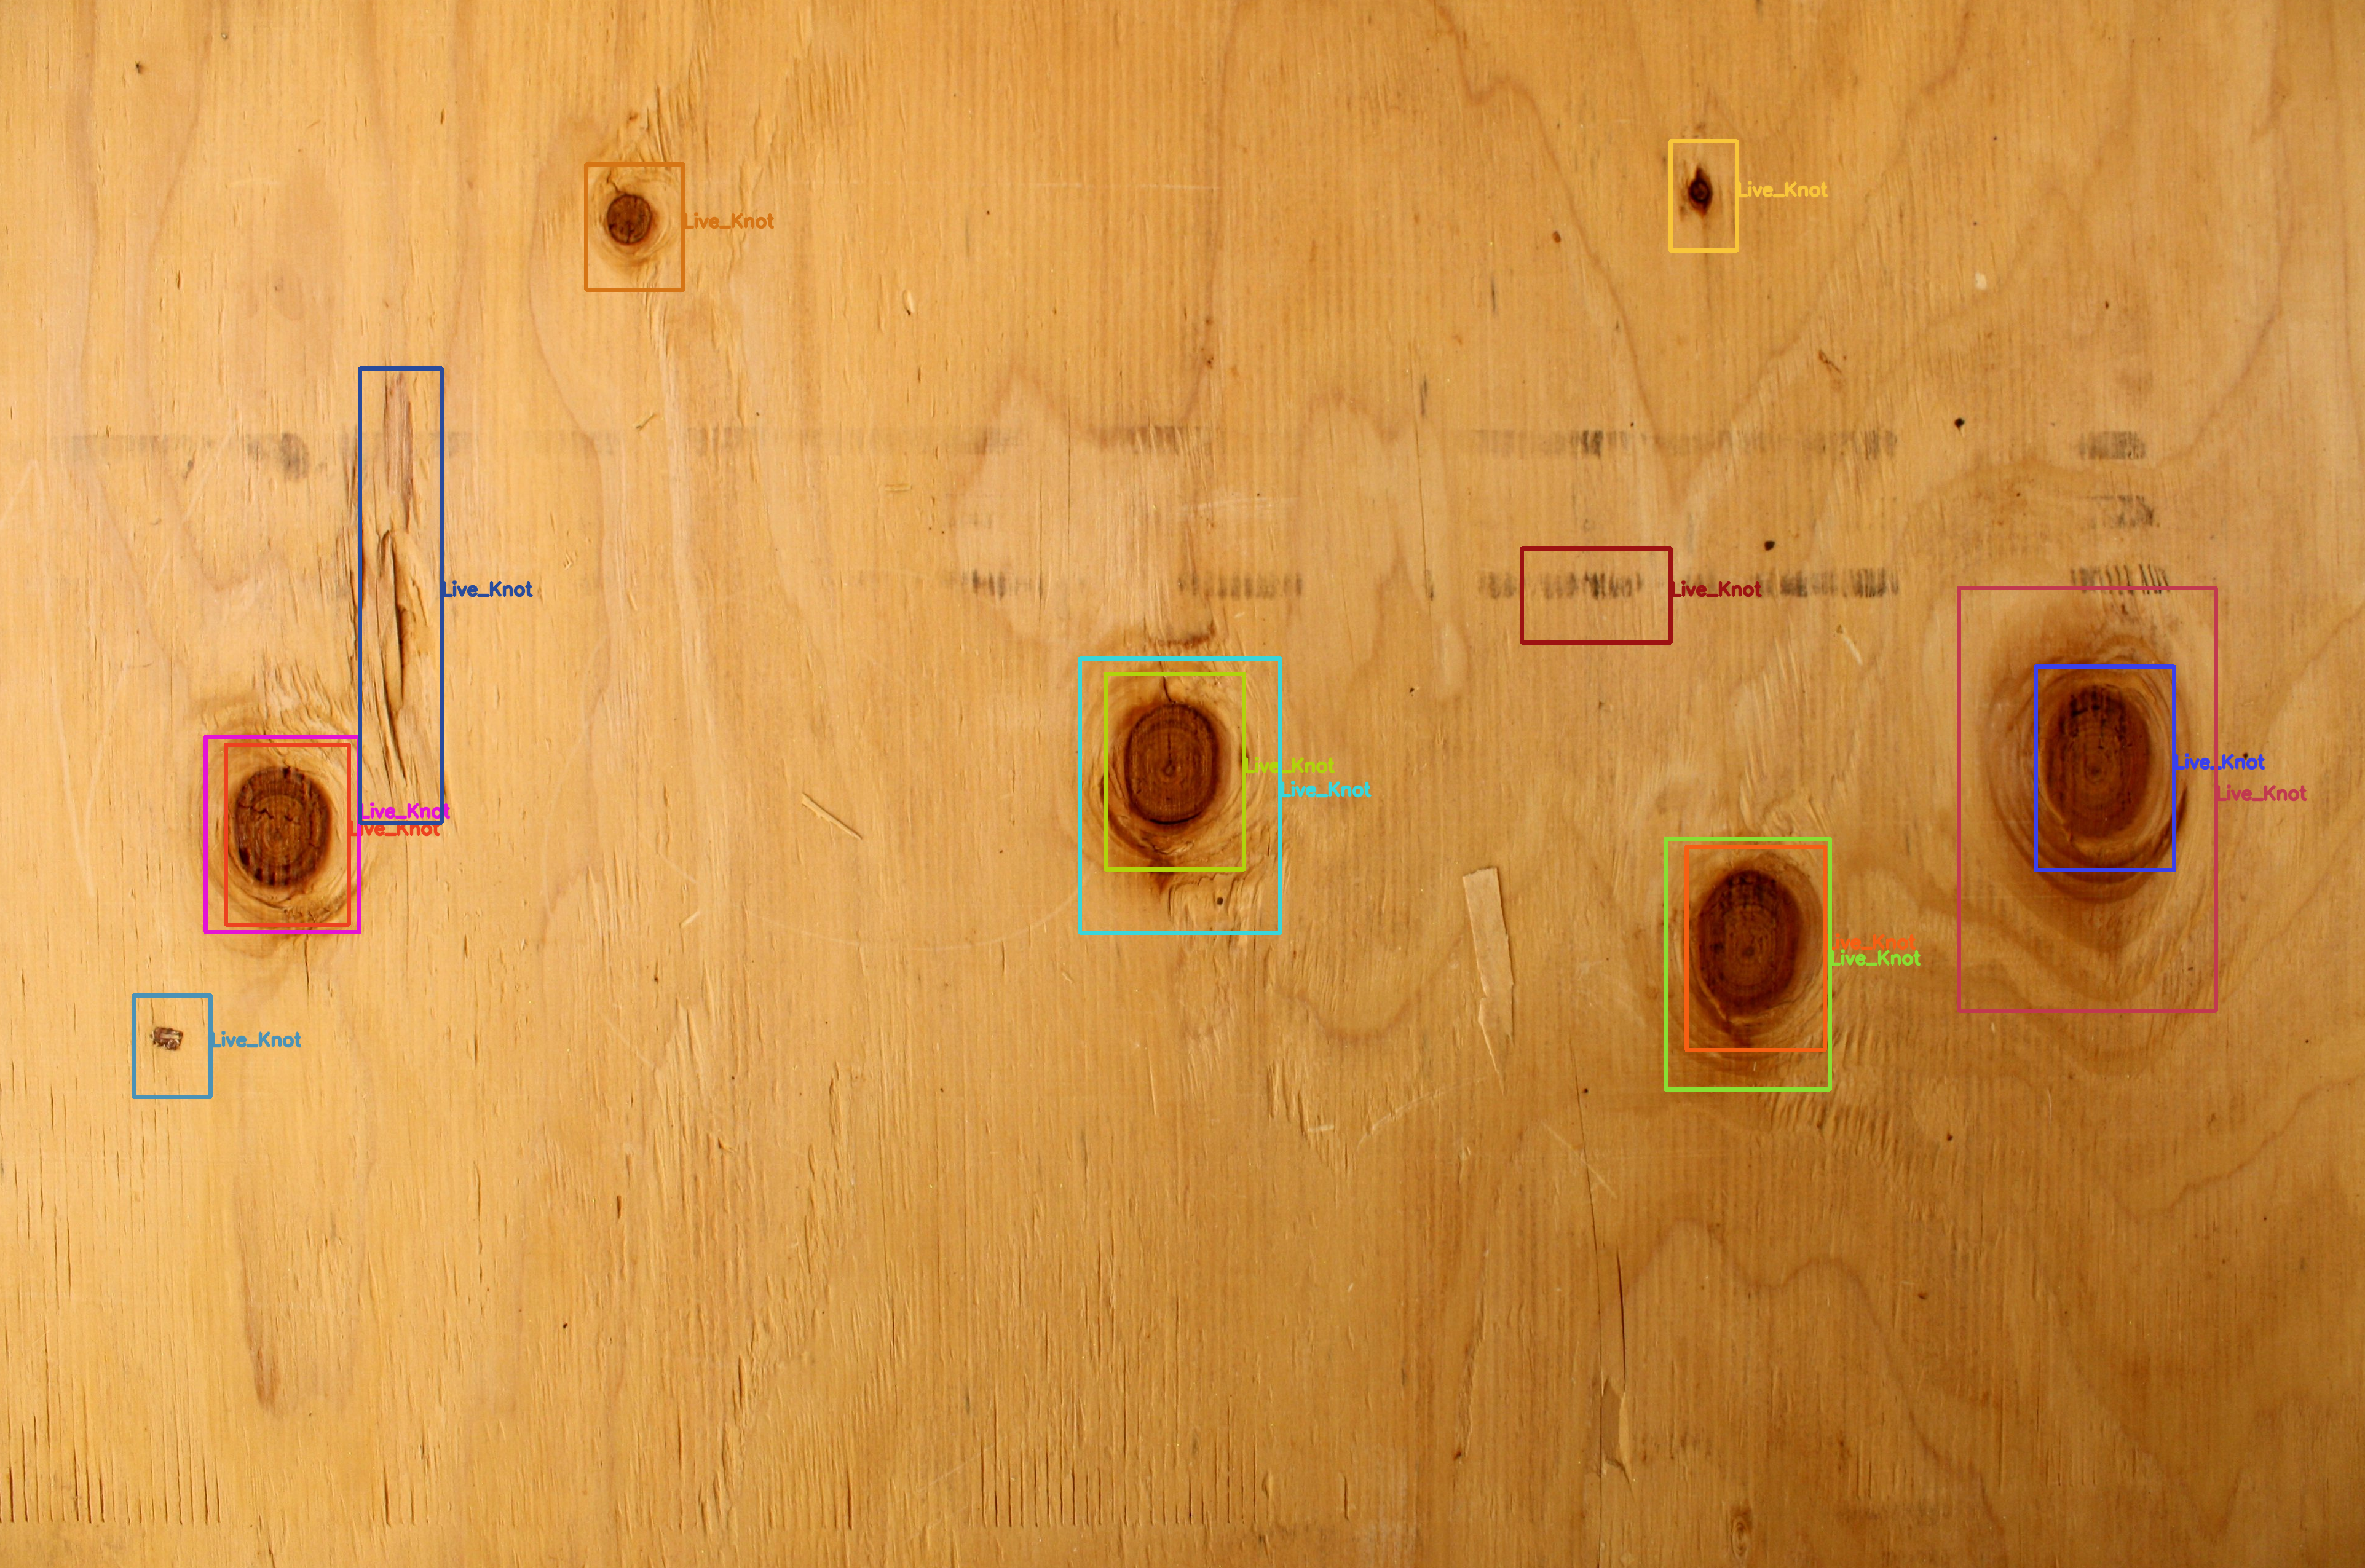
\includegraphics[scale=0.5]{3}
	    \caption{Розміщення даних у ROM.}
	\end{figure}
	
	\section*{Висновки}
	Під час виконання лабораторної роботи я навчився використовувати можливості лінкувальника та розташовувати дані за потрібними адресами. Створив фігурні літери свого імені (у латинській транскрипції) та логотип. Одержав бінарний файл, що містить ці дані і нічого більше.
	    
\end{normalsize}
\end{document}
